\section{Calcolo delle aree}

Abbiamo visto gli integrali come ``problema dell'antiderivata'': si cerca una funzione primitiva, la cui derivata \`e la funzione data. Si parla anche di operazione inversa della derivata. Guarda caso, il problema del calcolo delle aree \`e strettamente correlato al problema dell'integrazione.

Vogliamo calcolare l'area sotto una funzione. Sappiamo calcolarne ben poche, di base: quella dei rettangoli e quella del cerchio.

\begin{figure}[h]
\centering
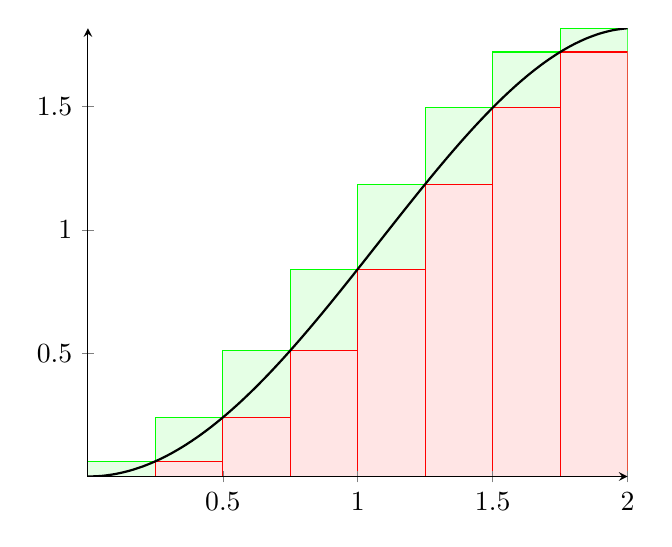
\begin{tikzpicture}[scale=1.0]
\begin{axis}[
    % xtick={0,...,1.5},ytick={0,...,1.5},
    % xmax=2,ymax=1.2,ymin=0,xmin=0,
    % enlargelimits=true,
    axis lines=middle,
    % clip=false,
    domain=0:2,
    axis on top
    ]

\addplot [draw=green, fill=green!10, const plot mark right, samples=9, domain=0:2]
    {x * sin(deg(x))}\closedcycle;
\addplot [draw=red, fill=red!10, ybar interval, samples=9, domain=0:2]
    {x * sin(deg(x))}\closedcycle;

\addplot[smooth, thick,domain=0:2,samples=40]{x * sin(deg(x))};
\end{axis}
\end{tikzpicture}
\caption{Somme di Riemann inferiori e superiori}
\end{figure}

Suddividiamo in un certo numero di rettangoli il sottografico della funzione. Disegnamo $n$ rettangoli, ciascuno con un area (data dalla base per l'altezza), e la somma delle aree \`e minore dell'area che vogliamo calcolare.

I punti scelti costituiscono una partizione dell'intervallo $[a,b]$. Se prendiamo una partizione pi\`u fitta, ottenendo quindi pi\`u rettangoli, la somma delle aree dei rettangoli \`e maggiore a quella precedente, ed \`e pi\`u vicina all'area che vogliamo calcolare.

Questa \`e l'idea di tal Cavalieri, il ``principio di esaustione''. Infittendo la partizione si approssima sempre meglio l'area sotto la curva.

Si pu\`o calcolare la somma delle aree dei rettangoli costruibili \emph{sopra} al grafico. L'area della somma di questi rettangoli \emph{contiene} l'area della funzione. In questo caso, infittendo la partizione, l'area diminuisce.

Vogliamo che queste due aree, quella sopra e quella sotto al grafico, siano, al limite, uguali. Se esiste un punto a cui queste due somme tendono, quel punto sar\`a proprio l'integrale.

\subsection{Somme di Riemann}

Consideriamo ora una funzione $f(x)$, e una partizione $P = \{ x_1, x_2, \ldots, x_n \}$ con $a = x_1 < x_2 < \ldots < x_{n-1} < x_n = b$.

Ora, per ogni coppia $[x_{i-1}, x_{i}]$ prendiamo due punti $l_i, u_i \in [x_{i-1}, x_{i}]$, tali che $f(l_i) \le f(x) \le f(u_i) \forall x \in [x_{i-1},x_{i}]$. I due punti $l_i$ e $u_i$ sono i punti di massimo e minimo della funzione nell'$i$-esimo intervallo.

Stiamo facendo l'ipotesi che in ciascuno di questi intervalli la funzione sia dotata di massimo e di minimo. Il teorema di Weierstrass ce lo garantisce, se la funzione \`e continua nell'intervallo.

Tenendo conto di queste notazioni, chiamiamo $L(P,f)$ la somma delle aree ``sotto'' la funzione, ossia:
\[
L(P,f) = \sum_{i = 1}^{n} f(l_i) \cdot (x_{i} - x_{i-1})
\]
Allo stesso modo, definiamo la somma $U(P,f)$ delle aree sopra la funzione:
\[
U(P,f) = \sum_{i = 1}^{n} f(u_i) \cdot (x_{i} - x_{i-1})
\]
\`E evidente che $L(P,f) \le U(P,f)$. Queste due quantit\`a si chiamano somme di Riemann, somma inferiore la prima e somma superiore la seconda.

Consideriamo due partizioni differenti, $P'$ e $P''$, vale sempre che $L(P',f) \le U(P'',f)$, anche se gli intervalli su cui ciascuna somma \`e basata sono differenti. Una somma fatta dal basso \`e sempre minore o uguale di una somma fatta dall'altro anche con una partizione differente.

Ora possiamo definire l'integrale definito, o integrale di Riemann.

\begin{defn}[Integrale di Riemann]
Se esiste un unico numero $I$ tale che $L(P',f) \le I \le U(P'',f) \forall P', P''$, allora $I$ sar\`a l'integrale di Riemann da $a$ a $b$:
\[
I = \int_{a}^{b} f(x) \dx
\]
\end{defn}
Questo \`e anche l'integrale definito, ma guai (per ora!) pensare di aver gi\`a visto il simbolo di integrale. \`E un simbolo con significato \emph{diverso} dal simbolo di integrale indefinito.

Come pu\`o succedere che non esista un unico numero $I$ che rispetta queste condizioni?

Consideriamo la funzione di Dirichlet, definita come segue:
\[
f(x) = 
\begin{cases}
1 \text{ se } x \in [0,1] \cap \rationals \\
0 \text{ se } x \notin [0,1] \setminus \rationals
\end{cases}
\]
Questa funzione non si pu\`o disegnare. Facciamo le somme di Riemann superiori e inferiori. In ogni intervallo abbiamo sia numeri razionali che numeri irrazionali. Il valore minimo della funzione \`e sempre 0, e il valore massimo \`e sempre 1, qualunque intervallo si scelga. Fra la somma inferiore e la somma superiore ci sono infiniti numeri, e non si pu\`o attribuire un'area al sottografico di questa funzione.

Se la funzione $f$ di cui vogliamo trovare l'area non \`e una funzione positiva nell'intervallo $[a,b]$ in cui cerchiamo l'area, che senso ha quello che stiamo facendo? Dobbiamo iniziare a parlare di \emph{area con segno}: consideriamo negativa un'area sotto l'asse delle $x$. I rettangoli che compongono la somma inferiore saranno pi\`u grandi dei rettangoli della somma superiore, ma attribuendogli un valore negativo la loro area resta minore dell'area dei rettangoli della somma superiore.

\begin{theorem}
\label{integrale_funzione_continua}
Se $f \in C^{0}([a,b])$ ($f$ \`e continua in $[a,b]$), allora esiste l'integrale definito $\int_{a}^{b} f(x) \dx$.
\end{theorem}

\begin{theorem}
Se $f \in C^{1}([a,b])$, ossia se $f$ \`e derivabile e $f'$ \`e continua in $[a,b]$, allora esiste l'integrale definito $\int_{a}^{b} f(x) \dx$.
\end{theorem}
Dimostrarlo per esercizio.

La scrittura $f \in C^{n} ([a,b])$ indica che la funzione $f$ \`e continua, \`e derivabile $n$ volte nell'intervallo $[a,b]$, e ognuna delle $n$ derivate \`e continua in $[a,b]$.

\begin{theorem} \label{integrabilita_riemann}
Usando le somme di Riemann si pu\`o stabilire se esiste l'integrale di Riemann.
\[
\exists \int_{a}^{b} f(x) \dx \iff \forall \epsilon > 0 \exists P \text{ t.c. } U(P,f) - L(P,f) < \epsilon
\]
Ossia, una funzione ha integrale di Riemann se e solo se la differenza fra le due somme (superiore e inferiore) pu\`o essere resa arbitrariamente piccola (con un'opportuna partizione).
\end{theorem}

\begin{oss}
Data una partizione $P$ di $[a,b]$, sia $c_i \in [x_{i-1},x_i]$ un punto qualunque nell'$i$-esimo intervallo determinato dalla partizione. Osserviamo che $f(l_i) \le f(c_i) \le f(l_i)$. Possiamo quindi scrivere che:
\[
L(P,f) = \sum_{i = 1}^{n} f(l_i) \cdot (x_{i} - x_{i - 1}) \le \sum_{i = 1}^{n} f(c_i) \cdot (x_{i} - x_{i - 1}) \le \sum_{i = 1}^{n} f(u_i) \cdot (x_{i} - x_{i - 1}) = U(P,f)
\]
\`E chiaro che se la funzione \`e integrabile, la somma di mezzo viene \emph{schiacciata} dalle altre due.
\end{oss}

Con questa osservazione possiamo tirare fuori una versione diversa del teorema \ref{integrabilita_riemann}.
\[
\int_{a}^{b} f(x) \dx = \lim_{\norm{P} \to 0} \sum_{i = 1}^{n} f(c_i) \cdot (x_i - x_{i - 1})
\]
La norma di $P$ ($\norm{P}$) \`e la massima lunghezza di un intervallo, ossia $\norm{P} = \max(x_i - x_{i-1})$.

% L'area del sottografico \`e l'area compresa fra il grafico e l'asse delle $x$. Se l'asse $x$ \`e sopra il grafico, l'area per convenzione ha segno negativo.

% L'integrale di una funzione dispari su un intervallo simmetrico rispetto all'asse $y$ \`e sempre nullo.

\subsection{Considerazioni sugli integrali definiti}

Per definizione, con gli integrali definiti vale:
\[
\int_{b}^{a} f(x) \dx = - \int_{a}^{b} f(x) \dx
\]
Facciamo qualche considerazione pi\`u o meno banale.
\begin{enumerate}
    \item Se $f(x) \le g(x)$ in $[a,b]$, allora:
    \[
    \int_{a}^{b} f(x) \dx \le \int_{a}^{b} g(x) \dx
    \]
    \item L'integrale definito \`e lineare:
    \[
    \int_{a}^{b} \left[ A \, f(x) + B \, g(x) \right] \dx =
    A \int_{a}^{b} f(x) \dx + B \int_{a}^{b} g(x) \dx
    \]
    Vederlo in maniera geometrica non \`e immediato. Ma abbiamo visto che le derivate sono lineari, visto che le derivate sono limiti e i limiti a loro volta sono lineari. Scriviamo questo integrale come limite, considerando una partizione $P = \{ x_1, x_2, \ldots, x_n \}$ e i punti $c_i \in [x_{i-1}, x_{i}]$:
    \[
    \lim_{\norm{P} \to 0} \sum_{i = 1}^{n} \left[ A \, f(c_i) + B \, g(c_i) \right] \cdot (x_{i} - x_{i-1})
    \]
    Ma il limite della combinazione lineare, abbiamo detto, \`e la combinazione lineare dei limiti:
    \[
    A \, \lim_{\norm{P} \to 0} \sum_{i = 1}^{n} f(c_i) \cdot (x_{i} - x_{i - 1}) +
    B \, \lim_{\norm{P} \to 0} \sum_{i = 1}^{n} g(c_i) \cdot (x_{i} - x_{i - 1})
    \]
    Questa quantit\`a \`e esattamente $A$ volte l'integrale definito di $f(x)$ pi\`u $B$ volte l'integrale definito di $g(x)$.
    \item Se $a < c < b$ ed esiste l'integrale definito $\int_{a}^{b} f(x) \dx$, allora:
    \[
    \int_{a}^{b} f(x) \dx = \int_{a}^{c} f(x) \dx + \int_{c}^{b} f(x) \dx
    \]
    \item Vale questa propriet\`a:
    \[
    \abs{\int_{a}^{b} f(x) \dx} \le \int_{a}^{b} \abs{f(x) \dx}
    \]
    \`E simile alla tipica disuguaglianza triangolare: $\abs{a + b} \le \abs{a} + \abs{b}$.
    \item Considerando integrali definiti su intervalli simmetrici rispetto all'asse $y$, se $f$ \`e pari vale che:
    \[
    \int_{-b}^{b} f(x) \dx = 2 \, \int_{0}^{b} f(x) \dx
    \]
    Se \`e dispari, vale invece che:
    \[
    \int_{-b}^{b} f(x) \dx = 0
    \]
\end{enumerate}

\subsubsection{Teorema del valor medio applicato agli integrali definiti}

Consideriamo un integrale definito di una funzione continua:
\[
\int_{a}^{b} f(x) \dx
\]
Siano, per il teorema di Weierstrass, $m = \min_{[a,b]} f(x)$ e $M = \max_{[a,b]} f(x)$. Possiamo minorare e maggiorare l'integrale definito come segue:
\[
\int_{a}^{b} m \dx \le \int_{a}^{b} f(x) \dx \le \int_{a}^{b} M \dx
\]
Si vede facilmente che $\int_{a}^{b} M \dx = M \cdot (b - a)$, e quindi che:
\[
m \cdot (b - a) \le \int_{a}^{b} f(x) \dx \le M \cdot (b - a) \implies
m \le \frac{1}{b - a} \int _{a}^{b} f(x) \dx \le M
\]
La funzione \`e continua per ipotesi, quindi assume tutti i valori fra minimo e massimo. Questo vuol dire che $\exists c \in (a,b)$ tale per cui:
\[
\frac{1}{b - a} \int_{a}^{b} f(x) \dx = f(c)
\]
Geometricamente, vuol dire che l'area sotto la funzione \`e uguale all'area del rettangolo alto $f(c)$ e largo quanto l'intervallo preso in esame, anche se non conosciamo dove sia il punto $c$.

\begin{exmp}
Consideriamo l'integrale definito $\int_{0}^{2} x \dx$, e la partizione $P_n$ dell'intervallo $[0,2]$ in sottointervalli ciascuno di lunghezza $\frac{2}{n}$. La differenza fra le somme inferiori e superiori di Riemann \`e:
\[
U(P_n, f) - L(P_n, f) = \sum_{i = 1}^{n} \left[ f(u_i) - f(l_i) \right] \cdot \frac{2}{n} = n \cdot \frac{4}{n^2}
\]
L'integrale definito di questa funzione, in questo intervallo, esiste: $\forall \epsilon > 0, \exists N_{\epsilon}$ tale per cui la differenza sopra \`e minore di $\epsilon$, per ogni $n \ge N_{\epsilon}$. Infatti basta che valga:
\[
n > \frac{4}{\epsilon}
\]
Si pu\`o poi far vedere quanto vale questo integrale definito, trovando i limiti delle somme inferiori o delle somme superiori.
\[
\int_{0}^{2} x \dx = 2 = \lim_{n \to \infty} U(P_n, f) = \lim_{n \to \infty} L(P_n, f)
\]
Infatti:
\[
\lim_{n \to \infty} U(P_n,f) = 
\lim_{n \to \infty} \sum_{i = 1}^{n} \frac{i \, 2}{n} \cdot \frac{2}{n} = \lim_{n \to \infty} \frac{4}{n^2} \cdot \sum_{i = 1}^{n} i =
\lim_{n \to \infty} \frac{\cancelto{2}{4}}{\cancel{n^2}} \cdot \frac{\cancel{n^2} + \cancelto{0}{n}}{\cancel{2}} = 2
\]
\end{exmp}

Salvo in casi particolari, l'unico modo per calcolare integrali definiti \`e attraverso l'approssimazione.

\section{Teorema fondamentale del calcolo}

Il teorema fondamentale del calcolo vale per ogni $f \in C^{0} ([a,b])$ (ossia per ogni funzione continua nell'intervallo chiuso e limitato $[a,b]$).

\begin{theorem}[Teorema fondamentale del Calcolo]
Sia $F(x) = \int_{a}^{x} f(t) \dx[t]$, per $a \le x \le b$, ossia la funzione che calcola l'area sotto il grafico della funzione $f$ dal punto $a$ al punto (variabile) $x$, allora:
\begin{enumerate}
    \item $\exists F'(x) = f(x)$
    \item $\forall G$ primitiva di $f$ in $[a,b]$, risulta che:
    \[
    \int_{a}^{b} f(x) \dx = G(b) - G(a) = \increment{\int f(x) \dx}_{a}^{b}
    \]
    L'ultima parte si legge ``incremento dell'integrale indefinito da $a$ a $b$''.
\end{enumerate}
\end{theorem}
Nella premessa, $x$ indica l'estremo superiore di integrazione, mentre la $t$ \`e una variabile muta di integrazione (e quindi non \`e minimamente rilevante la lettera che gli si associa).

La nozione di primitiva di una funzione e quella di area individuata dal grafo della funzione sono legate a doppio filo dal teorema fondamentale del Calcolo.

\begin{proof}
Calcoliamo la derivata della funzione $F(x)$.
\begin{align*}
\lim_{h \to 0} \frac{F(x + h) - F(x)}{h} = 
\lim_{h \to 0} \frac{1}{h} \, \left[ \int_{a}^{x+h} f(t) \dx[t] - \int_{a}^{x} f(t) \dx[t] \right] = \tag{per additivit\`a degli integrali} \\
= \lim_{h \to 0} \frac{1}{h} \, \left[ \cancel{\int_{a}^{x} f(t) \dx[t]} + \int_{x}^{x+h} f(t) \dx[t] - \cancel{\int_{a}^{x} f(t) \dx[t]} \right]
= \lim_{h \to 0} \frac{1}{h} \, \int_{x}^{x+h} f(t) \dx[t] = \tag{per il valor medio} \\
= \lim_{h \to 0} \frac{1}{h} \cdot f(c) \cdot (\cancel{x} + h - \cancel{x}) = \lim_{h \to 0} f(c) \cdot \frac{\cancel{h}}{\cancel{h}} = \lim_{h \to 0} f(c)
\end{align*}
Con $c \in [x, x+h]$, ma per $h \to 0$, si ha che $c \to x$, e quindi la derivata di $F(x)$ (che \`e la funzione che calcola l'area sotto $f(x)$) \`e proprio $f(x)$. 

Vediamo poi che se $G'(x) = f(x)$, allora $G(x) + c = \int_{a}^{x} f(t) \dx[t]$. Cosa segue da questo?

Prima di tutto, prendendo $x = a$, si ha che $G(a) + c = 0$, e quindi $c = - G(a)$.

Poi, prendendo $x = b$, abbiamo che $\int_{a}^{b} f(t) \dx[t] = G(b) + c = G(b) - G(a)$. E quindi una qualsiasi primitiva di $f(x)$ \`e la funzione che calcola l'area sotto il grafico di $f(x)$!
\end{proof}

\subsection{Integrali definiti e derivate}
\label{derivate_di_integrali}

Abbiamo detto che se $f \in C^0 ([a,b])$, ossia se \`e continua in $[a,b]$, allora $f$ \`e integrabile in $[a,b]$, e in particolare per ogni punto $x \in [a,b]$:
\[
F(x) = \int_{a}^{x} f(x) \dx
\]
Facendo variare il punto $x$ si ottiene una funzione che dipende da $x$. Il teorema fondamentale del calcolo integrale ci dice che questa funzione $F(x)$ \`e derivabile, e la derivata \`e la funzione integranda $f(x)$.

Cosa vuol dire questo?
\[
G(x) = \int_{a}^{x^2} f(t) \dx[t]
\]
Vuol dire che $G(x) = F(x^2)$. Infatti, se sostituiamo nell'equazione che segue $y$ con $x^2$, otteniamo la stessa cosa.
\[
F(y) = \int_{a}^{y} f(t) \dx[t]
\]
Se deriviamo $G(x)$ cosa succede?
\[
\deriv{x} G(x) = \deriv{x} F(x^2) = 2 \, x \, f(x^2)
\]
Basta applicare la regola di derivazione delle funzioni composte.

Una nota pedante sulla derivata delle funzioni composte. La derivata di una funzione, come $F(x^2)$, si scrive come la derivata della funzione ``esterna'' $F$ \emph{calcolata} in $x^2$ per la derivata della funzione ``interna'', $x^2$. Si scrive cos\`i:
\[
\deriv{x} F(x^2) = \left( \deriv{y} F \right) \left( x^2 \right) \cdot \deriv{x} \left( x^2 \right)
\]

\begin{exmp}
Guardiamo questa funzione:
\[
G(x) = \int_{0}^{\sin(x)} \frac{1}{1 + t^2} \dx[t]
\]
La sua derivata $G'(x)$ \`e:
\[
G'(x) = \frac{\cos(x)}{1 + \sin^2(x)} = \frac{\cancel{\cos(x)}}{\cos^{\cancel{2}}(x)} = \frac{1}{\cos(x)}
\]

Guardiamo questa:
\[
G(x) = \int_{a}^{\tan \left[ \log(1 + x^2) \right]} \arctan \left[ e^{t^2 + \cos(t)} \right] \dx[t]
\]
Non possiamo neanche lontanamente pensare di trovare l'integrale di questo mostro. Noi vogliamo solo calcolare $G'(x)$. Si prende la funzione integranda e la si calcola nell'estremo superiore, e la si moltiplica per la derivata dell'estremo superiore.
\begin{align*}
G'(x) &= \arctan \left[ e^{{\tan \left[ \log(1 + x^2) \right]}^2 + \cos \left( \tan \left[ \log(1 + x^2) \right] \right)} \right] \cdot \left[ \tan \left[ \log(1 + x^2) \right] \right]' = \\
&= \arctan \left[ e^{{\tan \left[ \log(1 + x^2) \right]}^2 + \cos \left( \tan \left[ \log(1 + x^2) \right] \right)} \right] \cdot \frac{1}{\cos^2 \left[ \log(1 + x^2) \right]} \cdot \frac{1}{1 + x^2} \cdot 2 \, x
\end{align*}

Questi esempi infami servono a capire cosa significa il teorema fondamentale del calcolo, ossia che l'integrale $\int_{a}^{x} f(t) \dx[t] = F(x)$ \`e tale che $F'(x) = f(x)$. Quindi la derivata di questo integrale \`e immediata:
\[
\deriv{x} \int_{a}^{x} \cos (\tan(1 + t^2)) \cdot e^{\arctan(\log(1+t^{2 \, \cos^2(t)}))} \dx[t] = 
\cos (\tan(1 + x^2)) \cdot e^{\arctan(\log(1+x^{2 \, \cos^2(x)}))}
\]
Per calcolare la derivata della funzione $F(x)$ non dobbiamo conosccere la funzione $F(x)$, perch\'e conosciamo la funzione $f(x)$.

E se volessimo derivare un integrale che ha delle funzioni in entrambi gli estremi di integrazione?
\[
G(x) = \int_{\tan(x^2)}^{e^{2x + \cos^2(x)}} \left[ t^a + \log(1 + t^2) \right] \dx[t]
\]
A esser precisi bisognerebbe dire che la $x$ \`e compresa fra $- \frac{\pi}{2}$ e $\frac{\pi}{2}$. Comunque, sappiamo come spezzare questo integrale:
\[
G(x) = \int_{0}^{e^{2x + \cos^2(x)}} \left[ t^a + \log(1 + t^2) \right] \dx[t] - \int_{0}^{\tan(x^2)} \left[ t^a + \log(1 + t^2) \right] \dx[t]
\]
Si possono scambiare gli estremi di integrazione invertendo il segno dell'integrale. Adesso sapppiamo come calcolare la derivata di $G(x)$.
\begin{align*}
G'(x) =& e^{2a \, x + a \, \cos^2(x)} + \log(1 + e^{4 \, x + 2 \, \cos^2(x)}) \cdot e^{2 \, x + \cos^2 (x)} \cdot \left( 2 - 2 \, \sin(x) \cos(x) \right) + \\
&-  {\tan(x^2)}^a + \log(1 + {\tan(x^2)}^2) \cdot \frac{1}{\cos^2(x)} \cdot 2 \, x
\end{align*}

In questo caso non abbiamo assolutamente modo di trovare la primitiva di $f(x)$:
\[
G(x) = \int_{\sin(x)}^{\cos^2(x)} e^{-t^2} \dx[t]
\]
Ma sappiamo sempre trovare la derivata di $G(x)$.
\[
G'(x) = e^{-{\left[ \cos^2(x) \right]}^2} \cdot (- 2 \sin(x) \cos(x)) - 
e^{-\sin^2(x)} \cdot \cos(x)
\]
\end{exmp}

Se adesso vogliamo tirare fuori un caso generale, possiamo scrivere che, dato questo integrale:
\[
G(x) = \int_{\alpha (x)}^{\beta (x)} f(t) \dx[t]
\]
la sua derivata \`e:
\[
G'(x) = f(\beta(x)) \cdot \beta'(x) - f(\alpha(x)) \cdot \alpha'(x)
\]
per il teorema fondamentale del calcolo.

\subsection{Funzioni continue a tratti}

Un esempio di funzione continua a tratti \`e la funzione parte intera.
\[
f(x) = \left[ x \right]
\]
Supponiamo ora di voler calcolare l'integrale:
\[
\int_{\frac{3}{2}}^{4} \left[ x \right] \dx
\]
\begin{figure}[h]
\centering
\begin{tikzpicture}
    \begin{axis}[
            xmin=0,xmax=5,
            ymin=0,ymax=5,
            axis x line=middle,
            axis y line=left,
            axis line style={->},
            % xlabel={$\reals$},
        ]
        \addplot[line width=2pt,-,domain=0:1]{0};
        \addplot[line width=2pt,-,domain=1:2]{1};
        \addplot[line width=2pt,-,domain=2:3]{2};
        \addplot[line width=2pt,-,domain=3:4]{3};
        \addplot[line width=2pt,-,domain=4:5]{4};
        \addplot[fill=black,only marks,mark=*]coordinates{(0,0)(1,1)(2,2)(3,3)(4,4)};
    \end{axis}
\end{tikzpicture}
\caption{La funzione ``parte intera''}
\end{figure}

La funzione non \`e continua, e non \`e continua neanche nell'intervallo [1,2]. \`E continua solo nell'intervallo [1,2) che ha un estremo non chiuso! Ma l'area sotto il rettangolo [1,2] \`e identica all'area sotto il rettangolo [1,2), poich\'e differiscono di un solo segmento.

Quindi l'integrale che abbiamo visto vale:
\[
\int_{\frac{3}{2}}^{4} \left[ x \right] \dx =
\int_{\frac{3}{2}}^{2} \left[ x \right] \dx +
\int_{2}^{3} \left[ x \right] \dx +
\int_{3}^{4} \left[ x \right] \dx
\]

\section{Integrali impropri}

Sappiamo calcolare l'integrale indefinito di:
\[
\int \log (x) \dx = x \, \log (x) - x + c
\]
Poi, $\forall a \ge 0$, sappiamo calcolare questo integrale definito:
\[
\int_{a}^{1} \log (x) \dx = - 1 - a \, \log (a) + a
\]
Facendo il limite per a che tende a $0^+$, vediamo che quest'area vale:
\[
\lim_{a \to 0^+} \int_{a}^{1} \log (x) \dx = -1
\]
Sappiamo calcolare qualunque area di questo tipo, $\forall a, b \ge 0$:
\[
\int_{a}^{b} \log (x) \dx
\]
Abbiamo parlato solo di intervalli $[a,b]$ chiusi e limitati. La cosa pi\`u estrema che abbiamo fatto \`e stato togliere un punto dall'estremo dell'intervallo. Ma in questo caso, se studiamo $\log (x)$ nell'intervallo $(0,1]$, la funzione \`e continua \emph{ma non} limitata.

Prendendo per\`o un qualunque $a \in (0,1]$, la funzione nel punto $a$ \`e sia continua che limitata. Facendo tendere $a$ a $0^+$ vediamo che l'area sotto la funzione \`e limitata, e tende a $-1$. La cosa rilevante \`e che abbiamo attribuito un'area limitata al grafico di una funzione su un insieme illimitato. Adesso possiamo ammettere questo:
\[
\int_{0}^{1} \log (x) \dx = -1
\]
Questo \`e un integrale improprio. Un integrale improprio \`e il limite di un integrale proprio.

\begin{exmp}
Quello che segue \`e un normale integrale definito, per $b \in \reals$.
\[
\int_{1}^{b} \frac{\diff x}{1 + x^2} = \arctan (b) - \frac{\pi}{4}
\]
Ma se facciamo il limite per $b \to \infty$, l'integrale diventa un integrale improprio.
\[
\lim_{b \to \infty} \int_{1}^{b} \frac{\diff x}{1 + x^2} = \frac{\pi}{2} - \frac{\pi}{4} = \frac{\pi}{4}
\]
\end{exmp}

\begin{exmp}
Questo \`e immediatamente riconoscibile come un integrale improprio:
\[
\int_{0}^{1} \frac{\diff x}{x}
\]
La funzione integranda, infatti, non \`e definita in uno degli estremi di integrazione (nello specifico, in 0). Quindi trovare un integrale simile vuol dire trovare questo integrale:
\[
\lim_{a \to 0^+} \int_{a}^{1} \frac{\diff x}{x} =
\lim_{a \to 0^+} \log(1) - \log(a) = 
- \lim_{a \to 0^+} \log(a) = \infty
\]
Qui abbiamo quindi una funzione illimitata su un intervallo limitato, e il suo integrale non esiste.
\end{exmp}

\begin{exmp}
Variazioni sullo stesso integrale improprio.
\[
\int_{1}^{\infty} \frac{\diff x}{x}
\]
Anche questo \`e improprio. Abbiamo una funzione integranda che (in $[1, \infty)$) \`e limitata, nonostante l'intervallo preso non lo sia.
\[
\lim_{b \to \infty} \int_{1}^{b} \frac{\diff x}{x} = \lim_{b \to \infty} \log(b) = \infty
\]
\end{exmp}

Quindi l'integrale definito di $\frac{1}{x}$ non esiste n\'e fra 0 e 1, n\'e fra 1 e $\infty$. $\frac{1}{x}$ \`e una funzione illimitata in 0 e all'infinito. Sar\`a sempre cos\`i, con tutte le funzioni non limitate?

\begin{exmp}
L'integrale che segue sembra simile ai casi precedenti, ma... 
\[
\int \frac{\diff x}{x^2} = - \frac{1}{x} + c
\]
Rifacciamo entrambi i ``test'' fatti prima.
\begin{align*}
\int_{0}^{1} \frac{\diff x}{x^2} \\
\int_{1}^{\infty} \frac{\diff x}{x^2}
\end{align*}
Sempre due integrali impropri. Ma vogliamo capire quale integrale converge e quale diverge.
\[
\lim_{a \to 0^+} \int_{a}^{1} \frac{\diff x}{x^2} =
\lim_{a \to 0^+} - 1 + \frac{1}{a} = \infty
\]
Diverge fra 0 e 1...
\[
\lim_{b \to \infty} \int_{1}^{b} \frac{\diff x}{x^2} =
\lim_{b \to 0^+} - \frac{1}{b} + 1 = 1
\]
E converge a 1 fra 1 e $\infty$.
\end{exmp}

\begin{exmp}
Vediamo un altro caso apparentemente simile ai precedenti. 
\[
\int \frac{\diff x}{\sqrt{x}} = 2 \, \sqrt{x} + c
\]
Quale integrale improprio converge, e quale diverge?
\[
\lim_{a \to 0^+} \int_{a}^{1} \frac{\diff x}{\sqrt{x}} =
\lim_{a \to 0^+} 2 - 2 \, \sqrt{a} = 2
\]
Converge (a 2) fra 0 e 1...
\[
\lim_{b \to \infty} \int_{1}^{b} \frac{\diff x}{\sqrt{x}} =
\lim_{b \to 0^+} 2 \, \sqrt{b} - 2 = \infty
\]
E diverge fra 1 e $\infty$.
\end{exmp}

\subsection{Funzioni razionali e integrali impropri}
\label{integrali_impropri_razionali}

Conosciamo l'integrale di questa funzione generica:
\[
\int \frac{\diff x}{x^p} = 
\begin{cases}
\dfrac{x^{-p + 1}}{- p + 1} + c & \text{ se } p \neq 1 \\
\abslog{x} + c & \text{ se } p = 1
\end{cases}
\]
Vogliamo studiare due integrali impropri a partire da questa funzione generica.
\begin{align*}
\int_{0}^{1} \frac{\diff x}{x^p} \qquad
\int_{1}^{\infty} \frac{\diff x}{x^p}
\end{align*}
\`E chiaro che, per $p$ negativo o nullo ($p \le 0$), il primo \`e un integrale proprio (la funzione, infatti, \`e continua e limitata anche in 0). I casi interessanti sono quelli per $p > 0$. Vogliamo capire per quali valori di $p$ questo integrale converge e per quali diverge.

Abbiamo visto che se $p = \frac{1}{2}$ il primo converge, il secondo diverge, mentre se $p = 2$ il primo diverge e il secondo converge.

Vediamo il primo integrale improprio nel caso generico, per $p \neq 1$:
\[
\int_{0}^{1} \frac{\diff x}{x^p} = 
\lim_{a \to 0^+} \int_{a}^{1} \frac{\diff x}{x^p} =
\lim_{a \to 0^+} \frac{1}{- p + 1} - \frac{a^{-p + 1}}{-p + 1}
\]
Ora, tutto dipende da $-p + 1$. Per a che tende a $0^+$, $a^n$ tende a $0$ se l'esponente \`e positivo, o a $\infty$ se l'esponente \`e negativo. Quindi:
\[
\lim_{a \to 0^+} \frac{1}{- p + 1} - \frac{a^{-p + 1}}{-p + 1} =
\begin{cases}
\dfrac{1}{- p + 1} & \text{ se } p < 1 \\
\infty & \text{ se } p > 1
\end{cases}
\]
Se $p < 1$, abbiamo che $-p > - 1 \implies - p + 1 > 0$.

Vediamo l'altro integrale.
\[
\int_{1}^{\infty} \frac{\diff x}{x^p} =
\lim_{b \to \infty} \int_{1}^{b} \frac{\diff x}{x^p} = 
\begin{cases}
\text{qualcosa} \in \reals & \text{ se } p > 1 \\
\infty & \text{ se } p \le 1
\end{cases}
\]

\subsubsection{Recap}

Nell'intervallo $\ocint{0}{1}$ vale questo:
\[
\int_{0}^{1} \frac{\diff x}{x^p} = 
\begin{cases}
\dfrac{1}{- p + 1} & \text{ se } p < 1 \\
\infty & \text{ se } p \ge 1
\end{cases}
\]
Nell'intervallo $\coint{1}{\infty}$ vale questo:
\[
\int_{1}^{\infty} \frac{\diff x}{x^p} =
\begin{cases}
\text{qualcosa} \in \reals & \text{ se } p > 1 \\
\infty & \text{ se } p \le 1
\end{cases}
\]
E basta.

\begin{exmp}
Basta integrali impropri di funzioni razionali.
\[
\int_{0}^{\infty} x \, e^{-x} \dx =
\lim_{b \to \infty} \int_{0}^{b} x \, e^{-x} \dx = 
\increment{\lim_{b \to \infty} -x \, e^{-x} - e^{-x}}_{0}^{b} =
\lim_{b \to \infty} -b \, e^{-b} - e^{-b} + 1 = + 1
\]
\end{exmp}

\begin{exmp}
Studiamo questo integrale improprio:
\[
\int_{- \infty}^{\infty} e^{-\abs{x}} \dx
\]
La funzione \`e pari, ed \`e limitata. La scriviamo come somma di due integrali impropri:
\begin{align*}
\int_{0}^{\infty} e^{-x} \dx + \int_{-\infty}^{0} e^{x} \dx =
2 \, \int_{0}^{\infty} e^{-x} \dx &= \\
2 \, \lim_{b \to \infty} \int_{0}^{b} e^{-x} \dx = 
\increment{2 \, \lim_{b \to \infty} - e^{-x}}_{0}^{b} = 
2 \, \lim_{b \to \infty} - e^{-b} + e^{0} &= 2
\end{align*}
\end{exmp}

\subsection{Criterio del confronto per determinare la convergenza}

Non tutti gli integrali sono simpatici, non di tutti gli integrali sappiamo trovare l'integrale indefinito.
\[
\int_{0}^{\infty} e^{-x^2} \dx
\]
Non serve a molto riscriverlo cos\`i:
\[
\lim_{b \to \infty} \int_{0}^{b} e^{-x^2} \dx
\]
perch\'e non sappiamo trovare l'integrale indefinito! Ma possiamo usare un criterio del confronto, dicendo prima questo:
\[
e^{-x^2} \le e^{-x}
\]
e quindi:
\[
\lim_{b \to \infty} \int_{0}^{b} e^{-x^2} \dx \le
\lim_{b \to \infty} \int_{0}^{b} e^{-x} \dx = 1
\]

Sono sempre e solo due le cose che si possono fare, per vedere se un integrale improprio converge o diverge:
\begin{enumerate}
    \item maggiorare l'integrale dato con un integrale che converge, e scoprire quindi che l'integrale dato converge, oppure
    \item minorare l'integrale dato con un integrale che diverge, e scoprire quindi che l'integrale dato diverge.
\end{enumerate}

\begin{exmp}
Scopriamo se questo integrale (improprio) converge o diverge.
\[
\int_{-1}^{0} \frac{e^x}{x+1} \dx
\]
\`E improprio, perch\'e per $x$ che tende a $-1$ la funzione integranda tende all'infinito. In 0 la funzione \`e definita (e vale 1).

Si pu\`o vedere che vale questa disuguaglianza, sapendo che $e^0$ vale 1:
\[
\frac{e^x}{x+1} \le \frac{1}{x+1} \text{ per } x \in \ocint{-1}{0}
\]
Infatti sappiamo che $e^x$ in $\ocint{-\infty}{0}$ \`e crescente, con massimo in $0$, e il massimo vale 1. Quindi $e^x$ in $\ocint{-\infty}{0}$ si maggiora con 1!

Per\`o \`e una maggiorazione inutile, visto che la funzione con cui abbiamo maggiorato la funzione integranda \emph{non ha} un integrale convergente.

Ma in $\ccint{-1}{0}$ la funzione $e^x$ ha il minimo in $-1$, e quel minimo \`e $e^{-1}$. Quindi la funzione integranda possiamo minorarla cos\`i:
\[
\frac{e^{-1}}{x+1} \le \frac{e^x}{x+1} \text{ per } x \in \ocint{-1}{0}
\]
La funzione con cui abbiamo minorato \`e simile alla funzione con cui abbiamo maggiorato prima (\`e la funzione di prima moltiplicata per la costante $e^{-1}$), quindi anche l'integrale di questa funzione diverge. Avendo minorato, in questo caso, abbiamo capito che l'integrale improprio iniziale \emph{diverge}.
\end{exmp}

C'\`e una certa disuguaglianza molto importante:
\[
0 \le \frac{\sin(x)}{x} \le 1
\]

\begin{exmp}
La disuguaglianza serve per determinare la convergenza di questo integrale:
\[
\int_{0}^{\frac{\pi}{2}} \frac{\sin(x)}{x^{\frac{7}{4}}} \dx
\]
Prima vediamo qualcosa di sbagliato, sapendo che vale sempre $\sin(x) \le 1$:
\[
\int_{0}^{\frac{\pi}{2}} \frac{\sin(x)}{x^{\frac{7}{4}}} \dx \le
\int_{0}^{\frac{\pi}{2}} \frac{\diff x}{x^{\frac{7}{4}}}
\]
Ma questo diverge. Non serve a niente maggiorare con qualcosa che diverge.

Invece possiamo maggiorarlo con qualcosa che converge:
\[
\int_{0}^{\frac{\pi}{2}} \frac{\sin(x)}{x^{\frac{7}{4}}} \dx =
\int_{0}^{\frac{\pi}{2}} \frac{\sin(x)}{x} \, \frac{\diff x}{x^{\frac{3}{4}}} \le
\int_{0}^{\frac{\pi}{2}} \frac{\diff x}{x^{\frac{3}{4}}}
\]
E quest'ultimo, per le regole viste nella sezione \ref{integrali_impropri_razionali}, converge.
\end{exmp}

\begin{exmp}
Questo integrale:
\[
\int_{1}^{\infty} \frac{x \, \arctan(x)^2}{x^3 + \log(x)} \dx
\]
Maggioriamo il numeratore e minoriamo il denumeratore, per maggiorare tutto l'integrale:
\[
\frac{x \, \arctan(x)^2}{x^3 + \log(x)} \le \frac{x \cdot \left( \frac{\pi}{2} \right)^2}{x^3}
\]
Questo \`e simile a un integrale del tipo $\frac{1}{x^2}$, che sappiamo convergere in $\coint{1}{\infty}$. A posto.
\end{exmp}














